% ######################## ROZDZIAŁ 1 ##########################
\chapter{Wstęp}
\label{cha:wstep}

\section{Wprowadzenie}
\label{sec:wprowadzenie}

W dzisiejszym świecie człowiek jest otoczony nowoczesną technologią. Trudno jest sobie wyobrazić egzystencję bez niej oraz jej ciągłego rozwoju opartego na tworzeniu coraz to lepszych i szybszych aplikacji czy narzędzi. Ich głównym zadaniem jest ułatwienie nam życia, ale również dostarczanie nam różnego rodzaju rozrywki. Trend nieustannego dążenia do perfekcji postawił przed nami problemy, z którymi ciężko sobie poradzić opierając się na znanych nam schematach przy użyciu klasycznych algorytmów. Czasami potrzebujemy, aby nasz kod był w stanie podejmować samodzielne decyzje, uczyć się na błędach, rozwiązywać problemy w taki sam sposób, jak ludzie. Dziedziną, która jest ściśle powiązana z tymi kwestiami, ich rozwiązywaniem oraz udoskonalaniem jest uczenie maszynowe, którego jedna z gałęzi jest wątkiem przewodnim niniejszej pracy.
    
    Uczenie maszynowe to dziedzina wchodząca w skład wielu innych obszarów nauki, takich jak informatyka czy statystyka. Jej głównym celem jest stworzenie systemu, który potrafi wykonać określone zadanie bez użycia doraźnych instrukcji, opierając się na wzorcach i wnioskowaniu. Systemu, przed którym będą stawiane zadania, z którymi mierzy się człowiek w jego codziennym życiu. Najczęściej kojarzy się to nam z robotami, które mają za zadanie ludziom pomagać lub niektórych sprawach ich wyręczać takich jak prowadzenie samochodu, robienie zakupów, przenoszenie obiektów z jednego miejsca na drugie. Jest to tylko niewielka część możliwości takich systemów ale należy pamiętać, że uczenie maszynowe to nie tylko roboty, lecz także algorytmy, które potrafią ewoluować, uczyć się i wykonywać pewne operacje lepiej, szybciej, efektywniej. Można je wykorzystać przy tworzeniu artykułów, które byłyby napisane bez naszego udziału lub ocenianiu treści najbardziej trafnych z punktu widzenia zwykłego człowieka. Zapotrzebowanie na tego typu programy jest bardzo duże i wciąż rosnące, z tego też względu postanowiliśmy się podjąć zadania postawionego w temacie naszej pracy.

    Celem jest stworzenie aplikacji, która będzie potrafiła kategoryzować treści ładowane dynamicznie. Dla dowolnej strony internetowej będziemy się starali wyciągnąć z niej najważniejsze informacje takie jak, m.in.  tytuły artykułów, treści artykułów czy komentarze. Uzyskamy to wykorzystując wiedzę na temat NLP, czyli przetwarzania języka naturalnego, które jest dziedziną łączącą takie obszary nauki, jak sztuczna inteligencja i językoznawstwo. W dalszej części tej pracy spotkamy się z opisem dotyczącym celów i założeń stawianych w naszym projekcie.


\section{Cel i~założenia projektu}
\label{sec:cel}

Celem niniejszej pracy jest opracowanie aplikacji, która będzie kategoryzować treści tekstowe dynamicznie ładowane na stronach internetowych. Aby osiągnąć zamierzony efekt należy zaprojektować i zaimplementować metody umożliwiające analizę tekstowych zbiorów danych. Praca będzie skoncentrowana na problemie kategoryzacji treści, a nie budowie samego narzędzia do pobierania treści dynamicznie ładowanych ze stron internetowych. Założeniem projektu jest dostępność przykładowych danych skategoryzowanych jako wartościowe i bezwartościowe (które sami arbitralnie przygotowaliśmy). Oczekiwanym produktem końcowym jest moduł aplikacji służący do kategoryzacji treści tekstowych.


% **********************
\section{Użytkownik końcowy}
\label{sec:uzytkownik}
% **********************

Prezentowany w niniejszej pracy system ma jedno podstawowe zadanie – kategoryzacja dynamicznie ładowanych treści ze stron internetowych. W dzisiejszych czasach, jak wiadomo, takie treści znajdują się praktycznie na każdej stronie internetowej. Wraz z postępem technicznym, wprowadza się do produkcji nowe, udoskonalone urządzenia, narzędzia i nowe technologie. To szczególnie dotyczy dziedziny nauki, jaką jest informatyka, która aktualnie jest jedną z najszybciej rozwijających się dyscyplin. Można pokusić się o stwierdzenie, iż nie da się już „normalnie" funkcjonować bez dostępu do tych technologii. Stąd nasza aplikacja jest skierowana do każdego użytkownika korzystającego z usług sieciowych. W jaki sposób można z niej korzystać? Głównym celem jest skategoryzowanie dynamicznie ładowanych treści. Działanie naszej aplikacji może przypominać działanie rozszerzeń dla przeglądarek internetowych umożliwających blokowanie reklam – tzw. \textit{adblocków}, jednakże jej zakres jest znacznie szerszy od tego typu aplikacji. 

\begin{figure}[h]
    \centering
    
\includegraphics[width=1\textwidth]{rys.1.1.adblock.png}
    \caption{Przykładowe działanie aplikacji „AdblockPlus”}
    \label{fig:mesh1}
\end{figure}

Przypomnijmy, adblock umożliwia filtrowanie treści reklamowych w postaci plików graficznych, animacji Flash czy wyskakujących okien z wyświetlanych stron internetowych (rys.~\ref{fig:mesh1}). Możliwe jest blokowanie całych serwisów, wybranych elementów strony, klas i identyfikatorów CSS wraz z wyszczególnieniem ich atrybutów. Możliwe jest także używanie wyrażeń regularnych co bardzo ułatwia tworzenie filtrów.

Nasz projekt niejako przypomina adblocka, ponieważ będzie niektóre dane klasyfikował jako „nieprzydatne”. Natomiast przewaga naszego produktu nad wcześniej wspomnianymi adblockami wynika z jego możliwości (co jest de facto jego głównym wymaganiem) klasyfikowania danych tekstowych, w wyniku czego jesteśmy w stanie obramować lub usunąć sekcję w dokumencie HTML na podstawie przypisanych kategorii do każdego z nich. Przykładowo osoba czytający dany artykuł chciałaby wyłącznie skupić się na jego treści - wtedy możemy wyłączyć wszystkie pozostałe zawartości, jak komentarze, czy przyciski przenoszące nas do innej części portalu. A więc z opisu funkcjonalności naszego produktu wprost wynika, że potencjalnym odbiorcą naszego produktu może się stać każdy użytkownik sieci Internet, który ma wolę ograniczenia zbędnych informacji wyświetlanych na stronach internetowych.

Początkowy zarys działania aplikacji został przedstawiony na rys.~\ref{fig:mesh2}.

\begin{figure}[h]
    \centering
    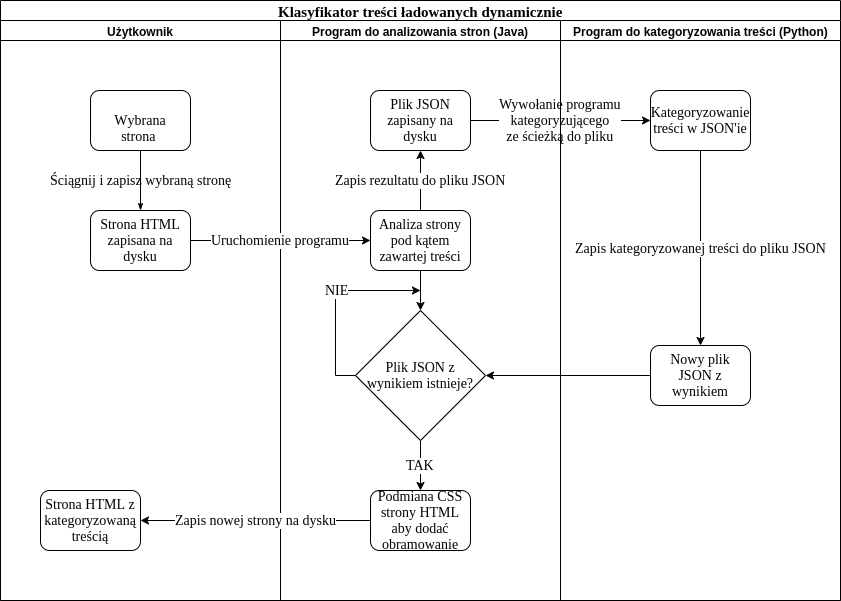
\includegraphics[width=1\textwidth]{rys.1.2.koncepcja.png}
    \caption{Klasyfikator treści ładowanych dynamicznie - początkowa koncepcja}
    \label{fig:mesh2}
\end{figure}


% **********************
\section{Technologia i koncepcja rozwiązania}
\label{sec:1.4.}
% **********************

Nasza praca bezpośrednio jest związana z tematyką natural language processing oraz machine learning. Dodatkowo, aby osiągnąć ten cel, musimy skorzystać z takich metod jak web crawling oraz web scraping. Na czym to polega?

Web crawler to program przeszukujący sieć WWW w celu zebrania informacji o strukturze i treściach znajdujących się na stronach internetowych. Niektóre przeglądarki używają takiego oprogramowania w celu indeksowania stron internetowych, dzięki czemu użytkownicy mogą skuteczniej wyszukiwać informacje. 
Natomiast web scraping to pozyskiwanie danych ze stron internetowych, np. za pomocą dostępu do sieci WWW. Metody te będą między innymi potrzebne do zgromadzenia danych wykorzystywanych w celu „nauczenia” naszego programu (modelu) poprawnego klasyfikowania danych do jednej z pięciu wyznaczonych klas (tytuł, treść artykułu, komentarz, menu, bezwartościowa treść). Metody te można łatwo zaimplementować w języku programowania Java, na co się zdecydowaliśmy. Wykorzystamy do tego biblioteki takie jak jsoup oraz gson które pomogą nam w analizie kodu źródłowego i zapisie jego treści w formacie JSON.

Kolejną wspomnianą techniką jest natural language processing, czyli dosyć szeroka dziedzina łącząca zagadnienia sztucznej inteligencji i językoznawstwa. Zajmuje się automatyzacją analizy, rozumienia, tłumaczenia i generowania języka naturalnego przez komputer. Jest ona jednym z rdzeni naszego produktu, który głównie polega na analizie tekstów oraz ich klasyfikacji, czyli przypisania ich do odpowiedniej kategorii. 

Ostatnią wspomnianą techniką jest machine learning, główny trzon naszego oprogramowania. Jest to dziedzina nauki dająca komputerom możliwość nauki nie będąc do tego zaprogramowanymi wprost.  Aby zrealizować wyżej wymienione cele, najbardziej słusznym wyborem wydaje się być język programowania Python. Jest on obecnie najczęściej wykorzystywany w dziedzinie sztucznej inteligencji, a to ze względu na mnogość bibliotek ułatwiających obliczenia matematyczne (na wektorach i macierzach), co jest główną składową tej dziedziny nauki. Przede wszystkim jednak, Python charakteryzuje się zwięzłością i czytelnością. Dzięki temu programiści mogą wkładać cały swój wysiłek w rozwiązywanie problemu ML zamiast skupiać się na technicznych niuansach języka. Mamy tutaj wiele gotowych modułów, które są testowane i używane od wielu lat, stąd też są bardzo dobrze udokumentowane. W projekcie korzystamy z bibliotek wbudowanych:
\begin{itemize}
\item argparse
\item pathlib
\item os
\end{itemize} 
oraz z bibliotek zewnętrznych:
\begin{itemize}
\item PyTorch
\item Flair
\end{itemize} 
Wszystkie one są bezpośrednio związane z tą tematyką i znacząco usprawnią pracę nad naszym zadaniem. Dodatkowo, będziemy korzystać również z metod analizy i wizualizacji dużych zbiorów danych w celu usystematyzowania rozwoju naszego oprogramowania.

% **********************
\section{Studium wykonalności}
\label{sec:1.5.}
% **********************

W naszym projekcie wykorzystujemy znajomość takich języków programowania jak Python oraz Java. Mamy w nich duże doświadczenie oraz wiemy jak łączyć oraz komunikować się między aplikacjami w wybranych językach. Każdy z nas ma swoje preferencje co do tego co chciałby włożyć w projekt i jakie rozwiązania zastosować. Wyzwaniem dla nas jest napisanie oraz nauczenie modelu opartego o NLP, gdyż jest to dla nas obszar bliżej niepoznany. Jak dotąd posiadaliśmy wiedzę jedynie z zakresu sieci neuronowych oraz tworzenia aplikacji przyjaznych użytkownikowi.
    
W przypadku klasyfikacji danych będziemy opierać się na bibliotece Flair, która ma przygotowane wstępne modele ułatwiające uczenie nowych, opartych na nich rozwiązań. Problemem staje się czas i sprzęt, który jest nam potrzebny do trenowania naszego klasyfikatora. W tym celu wykorzystamy prywatne komputery z dużą ilością RAM oraz kartą graficzną GPU pozwalającą na wykonywanie operacji związanych z uczeniem modelu.

Naszą pracę podzielimy ze względu na wygodę, elastyczność oraz większą znajomość w danej dziedzinie. Dlatego też wyznaczyliśmy dwa główne moduły projektu:
\begin{itemize}
\item \textbf{aplikacja do analizowania stron} – zastosowana do parsowania, modyfikowania oraz filtrowania pod kątem interesujących nas informacji, która będzie główną aplikacją.
\item \textbf{aplikacja do klasyfikowania treści} – odpowiedzialna za kategoryzację elementów znajdujących się na stronie a dokładnie danych znajdujących się w pliku JSON, który stanowił komunikację między obiema aplikacjami. Wykorzystywana wyłącznie jako pomoc do analizowania stron.
\end{itemize}
Każdy z nich odgrywa dużą rolę i jest niezbędny do poprawnego działania końcowego produktu. Dlatego tak istotne jest stworzenie dwóch aplikacji w jednym wspólnym celu jakim jest kategoryzowanie treści ładowanych dynamicznie na stronach internetowych. 

% **********************
\section{Analiza zagrożeń}
\label{sec:1.6.}
% **********************

Tworzenie takich aplikacji wiąże się z pewnym ryzykiem, z którym na wstępie musimy sobie poradzić, a jest nim:
\begin{itemize}[label=\textbullet]
\item \textbf{Aplikacja do parsowania stron może być niewydajna} – podczas analizowania strony pod kątem przeszukiwania tagów HTML zawierających jakąkolwiek treść wykorzystujemy bibliotekę jsoup, jednakże sprawdzanie każdej możliwości może być zbyt czasochłonne.

\item \textbf{Zebrane dane do uczenia mogą zawierać błędy albo być źle skategoryzowane} – podczas tworzenia modelu musimy zwrócić szczególną uwagę na zbiory testowe oraz to w jaki sposób je kategoryzujemy. Ponieważ zbieranie danych jest wykonywane ręcznie, gdyż każda strona ma inną sekwencję tagów prowadzącą do poszukiwanych przez nas treści to musimy wiedzieć czy nie istnieją jakieś wyjątki od reguły takie jak np. puste linie.

\item \textbf{Wybrane strony, z których zbieramy dane mogą mieć ich niewystarczającą ilość} – podczas wyborów stron musimy zwrócić uwagę na ilość artykułów, które możemy znaleźć na stronie, oraz na ich zawartość w celu znalezienia jak najbogatszego w treść źródła informacji.

\item \textbf{Wybrane strony mogą nam uniemożliwiać zbieranie danych} – wiele stron ma mechanizmy, które blokują ruch z jednego miejsca, który torpeduje ich zapytaniami (zabezpieczenia przed atakami DDoS). W tym celu musimy sprawdzić, które ze stron nie zablokują naszego połączenia podczas pobierania danych oraz musimy ustalić odstęp czasowy pomiędzy analizowanymi stronami. Ponadto wiele stron blokuje część treści dla programów niebędących przeglądarkami.

\item \textbf{Ilość zebranych danych będzie niewystarczająca, aby nauczyć nasz model} – początkowo nie wiedzieliśmy ile nasz model potrzebuje danych dla każdej kategorii, aby mógł się nauczyć klasyfikować dane. Zbiór testowy musiał być wielki, dlatego przyjęliśmy strategię uczenia na zestawach danych różnej wielkości, tak aby wiedzieć finalnie jak duży musi być zbiór treningowy.

\item \textbf{Wytrenowanie modelu będzie wymagało dużo czasu oraz dużych zasobów sprzętowych} – ponieważ był to nasz pierwszy kontakt z biblioteką Flair, nie wiedzieliśmy jak szybko jesteśmy w stanie wytrenować model z jej pomocą oraz w jaki sposób wykorzystuje dostępne zasoby sprzętowe. Dlatego też musieliśmy znaleźć urządzenie, które podoła naszym oczekiwaniom i będzie odporne na różnego rodzaju zdarzenia, niekoniecznie wynikające z pracy naszego programu.

\item \textbf{Dokładność kategoryzowania danych będzie niska} – czasami podczas trenowania różnych sieci, może dojść do ich przetrenowania, bądź wręcz przeciwnie - do ich niedouczenia, przez co dokładność i precyzja podczas ewaluacji na zbiorze testowym może być niska..

\item \textbf{Czas klasyfikowania danych może być zbyt długi} – podczas analizowania pliku JSON z danymi do sklasyfikowania może się okazać, że wydajność rozwiązania jest za niska.

\item \textbf{Nowo stworzona strona HTML z podmienionym plikiem CSS może nie wyświetlać poprawnie zawartości strony} – każda witryna posiada swoje osobne style CSS, które mogą kolidować z naszymi obramowaniami, co musimy wziąć pod uwagę jeśli chcemy, żeby prezentowane przez nas dane były dobrze wyświetlane.
\end{itemize}
Większość analizowanych problemów podczas pisania aplikacji można było w łatwy sposób rozwiązać lub ominąć. Te, które sprawiały najwięcej problemów wynikały z braku dobrej jakości urządzenia przeznaczonego do rozwiązywania tego typu zagadnień. Gdy już znaleźliśmy odpowiedni sprzęt mogliśmy rozpocząć pracę nad modelem, dlatego rozwój naszego projektu znacznie przyspieszył. Pozwoliło nam to na poszerzenie analizowanego problemu klasyfikacji o kolejne kategorie. Nie odbyłoby się to bez użyczenia nam superkomputera należącego do Naukowego Koła Robotyki i Sztucznej Inteligencji Uniwersytetu Jagiellońskiego, którego sympatykiem jest jeden z autorów tej pracy.
    
Parsowanie oraz zbieranie danych okazało się niezbyt wymagającym problemem, jednakże musieliśmy zwrócić uwagę na wiele szczegółów oraz detali, tak aby nasza końcowa aplikacja była jak najbardziej zbliżona do tego, co chcieliśmy uzyskać. Czas spędzony na gromadzeniu bazy danych się nieco wydłużył, co spowodowało przesunięcie innych etapów projektu na później. Mimo tego udało się nam dosyć szybko uporać z implementacją oraz uczeniem naszego modelu, dzięki czemu praca została ukończona na czas.

Największym atutem tej pracy jest fakt połączenia różnych aplikacji - do analizy stron w Javie oraz do klasyfikacji danych w Pythonie – ich komunikacji oraz finalnego efektu jakim jest obramowanie treści na stronie kolorowymi ramkami odpowiadającymi różnym kategoriom, które zostały im przypisane. Było to także dla nas miłe zaskoczenie, że trud włożony w wykonaną pracę opłacił się i jest dobrym pomysłem na późniejsze udostępnienie aplikacji jako część większego projektu opartego o klasyfikowanie stron oraz interpretację informacji na nich zawartych.

%\begin{enumerate}%[label=$\dot$]
%\item[\textbullet] liczba zdjęć reprezentujących niską wytrzymałość wzrosła z~65 do 1337,
%\end{enumerate}
% ^^^^ RÓWNOWAŻNE \/ \/ \/
%\begin{itemize}
%\item[\textbullet] liczba zdjęć reprezentujących niską wytrzymałość wzrosła z~65 do 1337,
%\end{itemize}

